% !TeX program = xelatex
\documentclass[a4paper,10pt]{article}

% ============================================================================
% សន្លឹកកិច្ចការសិស្សបំពេញចន្លោះ ស-ខ្មៅ និងប្លង់ក្ដារខៀន/ចម្លើយគ្រូ (គ្មាន LCD / គ្មានកន្ត្រៃ)
% មេរៀនទី៣ (២.៦)៖ ការប្រាក់សមាស — ត្រូវគ្នា ១០០% នឹង LS_Plan_INT326.tex
% ============================================================================
\usepackage[a4paper, left=1.0cm, right=1.0cm, top=0.75cm, bottom=1.00cm, footskip=0.52cm]{geometry}
\usepackage{amsmath}
\usepackage{unicode-math}
\usepackage{fontspec}
\usepackage{array, colortbl}
\usepackage[table]{xcolor}
\usepackage{enumitem}
\usepackage{pifont}
\usepackage{fancyhdr}
\usepackage{lastpage}
\usepackage{tikz}
\usepackage[most]{tcolorbox}
\usetikzlibrary{calc, arrows.meta, decorations.pathreplacing, positioning, babel}

\makeatletter
\let\@expl@@@mark@update@singlecol@structures@@\relax
\makeatother

\providecommand{\NGSFindFonts}{%
  \IfFileExists{C:/Windows/Fonts/cambria.ttc}{%
    \def\NGSSysPath{C:/Windows/Fonts/}%
    \def\NGSUserPath{C:/Users/KIT/AppData/Local/Microsoft/Windows/Fonts/}%
  }{%
    \IfFileExists{./fonts/KhmerOSsiemreap.ttf}{\def\NGSSysPath{./fonts/}\def\NGSUserPath{./fonts/}}{%
    \IfFileExists{../fonts/KhmerOSsiemreap.ttf}{\def\NGSSysPath{../fonts/}\def\NGSUserPath{../fonts/}}{%
    \IfFileExists{../../fonts/KhmerOSsiemreap.ttf}{\def\NGSSysPath{../../fonts/}\def\NGSUserPath{../../fonts/}}{%
    \IfFileExists{../../../fonts/KhmerOSsiemreap.ttf}{\def\NGSSysPath{../../../fonts/}\def\NGSUserPath{../../../fonts/}}{%
    \IfFileExists{../../../../fonts/KhmerOSsiemreap.ttf}{\def\NGSSysPath{../../../../fonts/}\def\NGSUserPath{../../../../fonts/}}{%
    \IfFileExists{../../../../../fonts/KhmerOSsiemreap.ttf}{\def\NGSSysPath{../../../../../fonts/}\def\NGSUserPath{../../../../../fonts/}}{%
    \IfFileExists{../../../../../../fonts/KhmerOSsiemreap.ttf}{\def\NGSSysPath{../../../../../../fonts/}\def\NGSUserPath{../../../../../../fonts/}}{%
      \def\NGSSysPath{../../../../../../../fonts/}\def\NGSUserPath{../../../../../../../fonts/}%
    }}}}}}}%
  }%
}
\NGSFindFonts

\setmathfont[Path={\NGSSysPath}, FontIndex=1, Scale=1.02]{cambria.ttc}
\defaultfontfeatures{Ligatures=TeX}

\setmainfont[
  Path={\NGSUserPath}, Extension=.ttf, Script=Khmer,
  BoldFont={KhmerOSsiemreap}, BoldFeatures={FakeBold=1.8},
  ItalicFont={KhmerOSsiemreap}, ItalicFeatures={FakeSlant=0.25},
  BoldItalicFont={KhmerOSsiemreap}, BoldItalicFeatures={FakeBold=1.8, FakeSlant=0.25}
]{KhmerOSsiemreap}

\newfontfamily\muol[Path={\NGSUserPath}, Extension=.ttf, Script=Khmer]{KhmerOSmuollight}
\newfontfamily\TimesEn[Path={\NGSSysPath}, Extension=.ttf, BoldFont={timesbd}, ItalicFont={timesi}, BoldItalicFont={timesbi}]{times}
\newfontfamily\CalibriFont[Path={\NGSSysPath}, Extension=.ttf]{calibri}

\XeTeXlinebreaklocale "km"
\XeTeXlinebreakskip = 0pt plus 1pt minus 0.1pt

\definecolor{panelgray}{gray}{0.94}
\definecolor{headgray}{gray}{0.85}
\definecolor{midgray}{gray}{0.76}

\pagestyle{fancy}
\fancyhf{}
\renewcommand{\headrulewidth}{0pt}
\fancyfoot[L]{\fontsize{7.4pt}{9.5pt}\selectfont អនុវិទ្យាល័យព្រះក្រសាំង \en{|} គ្រូ៖ ហុក ប៊ុនថែន \en{|} មេរៀនទី៣ (២\en{.}៦) ការប្រាក់សមាស \en{|} ថ្ងៃពុធ ទី២៥ ខែវិច្ឆិកា ឆ្នាំ២០២៦}
\fancyfoot[R]{\fontsize{7.8pt}{10pt}\selectfont ទំព័រ \en{\thepage\ / \pageref{LastPage}}}

\setlength{\parindent}{0pt}
\setlength{\parskip}{0pt}
\setlength{\tabcolsep}{4pt}

\newcommand{\en}[1]{{\TimesEn #1}}
\newcommand{\enbf}[1]{{\TimesEn\bfseries #1}}
\newcommand{\unit}[1]{\,\text{\en{#1}}}
\newcommand{\riel}{\,\text{៛}}
\newcommand{\usd}{\,\text{\en{\$}}}
\newcommand{\cnum}[1]{\mbox{\fontsize{10pt}{12pt}\selectfont\ding{\numexpr181+#1\relax}}}
\newcommand{\chkbox}{\tikz[baseline=-0.15ex]\draw[black, line width=0.85pt, fill=white] (0,0) rectangle (0.24cm,0.24cm);}
\newcommand{\ansbox}[1][1.75cm]{\,\tikz[baseline=-0.65ex]\draw[black, line width=0.65pt, fill=white] (0,0) rectangle (#1, 0.42cm);\,}
\newcommand{\dotline}[1][2.2cm]{\makebox[#1]{\dotfill}}

\newcommand{\pagebanner}[2]{%
  \begin{tcolorbox}[
    enhanced, sharp corners, colback=headgray, colframe=black,
    boxrule=1.05pt, boxsep=1pt, top=2.5pt, bottom=2.5pt, left=6pt, right=6pt,
    after skip=3.5pt
  ]
    {\muol\fontsize{9.0pt}{13.2pt}\selectfont #1}\hfill{\fontsize{8.0pt}{11.2pt}\selectfont\textbf{#2}}
  \end{tcolorbox}%
}

\newcommand{\secstrip}[2]{%
  \vspace{3pt}%
  \begin{tcolorbox}[
    enhanced, sharp corners, colback=panelgray, colframe=black,
    boxrule=0.8pt, boxsep=0.8pt, top=2pt, bottom=2pt, left=5pt, right=5pt,
    after skip=3pt
  ]
    {\muol\fontsize{8.5pt}{12.2pt}\selectfont #1}\hfill{\fontsize{7.8pt}{10.8pt}\selectfont\textit{#2}}
  \end{tcolorbox}%
}

\newcolumntype{L}[1]{>{\raggedright\arraybackslash}p{#1}}
\newcolumntype{C}[1]{>{\centering\arraybackslash}p{#1}}

\begin{document}
\fontsize{9.5pt}{14.5pt}\selectfont

% ============================================================================
% ទំព័រទី ១៖ សន្លឹកកិច្ចការសិស្ស (ផ្នែកមុខ៖ E1 -> E2 -> E3)
% ============================================================================
\pagebanner{សន្លឹកកិច្ចការសិស្ស \enbf{(}២\enbf{.}៦ ការប្រាក់សមាស\enbf{)} \enbf{--} ផ្នែកមុខ}{ថ្នាក់ទី៨ \en{|} សៀវភៅគោល ទំ.៣៧--៣៨}

\begin{tcolorbox}[
  enhanced, sharp corners, colback=white, colframe=black,
  boxrule=0.8pt, boxsep=1.5pt, top=3.5pt, bottom=3.5pt, left=5pt, right=5pt,
  after skip=4pt
]
  \fontsize{9.0pt}{13.0pt}\selectfont
  \textbf{ឈ្មោះសិស្ស៖} \dotline[4.3cm] \quad
  \textbf{សមាជិកក្រុម៖} \dotline[4.3cm] \quad
  \textbf{ថ្នាក់ទី៖} ៨\dotline[0.9cm] \quad
  \textbf{ក្រុមទី៖} \dotline[1.0cm]
\end{tcolorbox}

% --- E1 Engage ---
\secstrip{ផ្នែកទី ១ \enbf{(E1 - Engage)} ៖ បេសកកម្មគណនីសន្សំភ្លោះ \enbf{A} និង \enbf{B} ($1\,000\,000\riel$, $10\%$/ឆ្នាំ, $2$ ឆ្នាំ)}{រយៈពេល ៣ នាទី (គូស \ding{51} ក្នុង \chkbox)}

\begin{tcolorbox}[
  enhanced, sharp corners, colback=white, colframe=black,
  boxrule=0.8pt, boxsep=2pt, top=3.5pt, bottom=3.5pt, left=6pt, right=6pt
]
  បងប្អូនភ្លោះពីរនាក់ដាក់ប្រាក់ $1\,000\,000\riel$ ម្នាក់ រយៈពេល $2$ ឆ្នាំ ដោយអត្រា $10\%$ ក្នុង ១ ឆ្នាំ ៖ គណនី \en{A} ដកការប្រាក់រាល់ចុងឆ្នាំបានសរុប $200\,000\riel$ ឯគណនី \en{B} ទុកការប្រាក់ឆ្នាំទី១ បូកចូលប្រាក់ដើមសម្រាប់ឆ្នាំទី២!\\[2pt]
  $\bullet$ \textbf{ការទស្សន៍ទាយលើគណនី \en{B}៖} \quad
  \chkbox\ បាន $200\,000\riel$ ដូចគ្នា \qquad
  \chkbox\ បាន $210\,000\riel$ (ច្រើនជាង \en{A}!)\\[2pt]
  $\bullet$ \textbf{ហេតុផលខ្លី៖} តើប្រាក់ដើមនៅដើមឆ្នាំទី២ នៃគណនី \en{B} ឡើងដល់ប៉ុន្មានរៀល? \dotline[3.0cm] $\riel$ ។
\end{tcolorbox}

\vfill

% --- E2 Explore ---
\secstrip{ផ្នែកទី ២ \enbf{(E2 - Explore)} ៖ តារាងព្រួញបន្តប្រាក់ដើមប្រចាំឆ្នាំ (ទំ.៣៧--៣៨)}{រយៈពេល ១១ នាទី}

\textbf{សកម្មភាព ១ (\en{E2-A} — ៥ នាទី)៖ ឧទាហរណ៍មីងសៅដាក់ប្រាក់ $P_1 = 8\,000\,000\riel$, អត្រា $R = 15\%$/ឆ្នាំ, រយៈពេល $2$ ឆ្នាំ (ទំ.៣៧)}

\begin{tcolorbox}[
  enhanced, sharp corners, colback=white, colframe=black,
  boxrule=0.8pt, boxsep=2pt, top=3.5pt, bottom=3.5pt, left=6pt, right=6pt
]
  \centering
  {\renewcommand{\arraystretch}{1.28}
  \begin{tabular}{|C{2.0cm}|L{4.2cm}|L{5.6cm}|L{5.2cm}|}
    \hline
    \cellcolor{headgray}\textbf{ឆ្នាំទី} &
    \cellcolor{headgray}\textbf{ប្រាក់ដើមដើមឆ្នាំ ($P_k$)} &
    \cellcolor{headgray}\textbf{ការប្រាក់ប្រចាំឆ្នាំ ($I_k = P_k\times \frac{15}{100}$)} &
    \cellcolor{headgray}\textbf{ប្រាក់សរុបចុងឆ្នាំ ($A_k = P_k + I_k$)} \\
    \hline
    ឆ្នាំទី $1$ & $P_1 = 8\,000\,000\riel$ & $I_1 = 8\,000\,000\times \frac{15}{100} = 1\,200\,000\riel$ & $A_1 = 9\,200\,000\riel \ (\searrow P_2)$ \\
    \hline
    ឆ្នាំទី $2$ & $P_2 =$ \dotline[2.4cm] $\riel$ & $I_2 =$ \dotline[2.2cm] $\times \frac{15}{100} =$ \dotline[1.9cm] $\riel$ & $A_2 =$ \dotline[2.6cm] $\riel$ \\
    \hline
  \end{tabular}}\\[3pt]
  \raggedright $\implies$ \textbf{ការប្រាក់សមាសសរុប $2$ ឆ្នាំ៖} $I_{\text{សមាស}} = I_1 + I_2 = 1\,200\,000 +$ \dotline[2.0cm] $=$ \ansbox[2.2cm] $\riel$
\end{tcolorbox}

\vspace{3pt}
\textbf{សកម្មភាព ២ (\en{E2-B} — ៦ នាទី)៖ លំហាត់គំរូទី ១ — ទ្រាចាន់ចងការប្រាក់ឱ្យមីងស្រី $P_1 = 3\,000\,000\riel$, $R = 20\%$, $3$ ឆ្នាំ (ទំ.៣៧--៣៨)}

\begin{tcolorbox}[
  enhanced, sharp corners, colback=white, colframe=black,
  boxrule=0.8pt, boxsep=2pt, top=3.5pt, bottom=3.5pt, left=6pt, right=6pt
]
  \centering
  {\renewcommand{\arraystretch}{1.26}
  \begin{tabular}{|C{2.0cm}|L{4.2cm}|L{5.6cm}|L{5.2cm}|}
    \hline
    \cellcolor{headgray}\textbf{ឆ្នាំទី} &
    \cellcolor{headgray}\textbf{ប្រាក់ដើមដើមឆ្នាំ ($P_k$)} &
    \cellcolor{headgray}\textbf{ការប្រាក់ប្រចាំឆ្នាំ ($I_k = P_k\times \frac{20}{100}$)} &
    \cellcolor{headgray}\textbf{ប្រាក់សរុបចុងឆ្នាំ ($A_k = P_k + I_k$)} \\
    \hline
    ឆ្នាំទី $1$ & $P_1 = 3\,000\,000\riel$ & $I_1 = 600\,000\riel$ & $A_1 = 3\,600\,000\riel \ (\searrow P_2)$ \\
    \hline
    ឆ្នាំទី $2$ & $P_2 = 3\,600\,000\riel$ & $I_2 =$ \dotline[2.4cm] $\riel$ & $A_2 =$ \dotline[2.5cm] $\riel \ (\searrow P_3)$ \\
    \hline
    ឆ្នាំទី $3$ & $P_3 =$ \dotline[2.4cm] $\riel$ & $I_3 =$ \dotline[2.4cm] $\riel$ & $A_3 =$ \dotline[2.5cm] $\riel$ \\
    \hline
  \end{tabular}}\\[3pt]
  \raggedright $\implies$ \textbf{ការប្រាក់សមាសសរុប $3$ ឆ្នាំ៖} $I_{\text{សមាស}} = I_1 + I_2 + I_3 =$ \ansbox[2.4cm] $\riel$
\end{tcolorbox}

\vfill

% --- E3 Explain ---
\secstrip{ផ្នែកទី ៣ \enbf{(E3 - Explain)} ៖ ក្បួនគណនាការប្រាក់សមាស និងធនាគារហេតុផល \enbf{B\&W}}{រយៈពេល ៦ នាទី}

\begin{tcolorbox}[
  enhanced, sharp corners, colback=white, colframe=black,
  boxrule=0.85pt, boxsep=2pt, top=3.5pt, bottom=3.5pt, left=6pt, right=6pt
]
  $\bullet$ \textbf{និយមន័យ (ទំ.៣៧)៖} រាល់ដំណាច់ដំណាក់ គេយកការប្រាក់កន្លងទៅបូកបន្ថែមលើប្រាក់ដើម បាន\textbf{ប្រាក់ដើមថ្មី}៖ \quad
  $P_{k+1} = P_k + \dotline[1.0cm]$ \quad និង \quad
  $I_{\text{សមាស}} = I_1 + I_2 + \dots + I_n = A_n - \dotline[1.0cm]$\\[4pt]
  \tikz\draw[black, dashed, line width=0.5pt] (0,0) -- (18.4cm,0);\\[3pt]
  \fontsize{8.8pt}{12.8pt}\selectfont
  \textbf{ធនាគារហេតុផល (\en{Warrant Bank})៖} \quad
  \cnum{1} \textbf{បន្តដើមថ្មី៖} $P_{\text{ថ្មី}} = P_{\text{ចាស់}} + I_{\text{មុន}}$ \quad
  \cnum{2} \textbf{បូកសរុបគ្រប់ដំណាក់៖} $I_{\text{សមាស}} = I_1 + \dots + I_n$\\
  \cnum{3} \textbf{បន្តដើមប្រចាំឆមាស៖} $1\text{ ឆ្នាំ} = 2\text{ ឆមាស}$ ($T = \frac{1}{2}$ ឆ្នាំ ក្នុង ១ ឆមាស) \quad
  \cnum{4} \textbf{ប្រាក់សរុបចុងក្រោយ៖} $A_n = P_1 + I_{\text{សមាស}}$
\end{tcolorbox}

% ============================================================================
% ទំព័រទី ២៖ សន្លឹកកិច្ចការសិស្ស (ផ្នែកខាងខ្នង៖ E4 -> E5 -> កិច្ចការផ្ទះ)
% ============================================================================
\clearpage
\pagebanner{សន្លឹកកិច្ចការសិស្ស \enbf{(}២\enbf{.}៦ ការប្រាក់សមាស\enbf{)} \enbf{--} ផ្នែកខាងខ្នង}{ថ្នាក់ទី៨ \en{|} សៀវភៅគោល ទំ.៣៨, ៤២}

% --- E4 Elaborate ---
\secstrip{ផ្នែកទី ៤ \enbf{(E4 - Elaborate)} ៖ លំហាត់គំរូទី ២ — ការប្រាក់សមាសប្រចាំឆមាស (ទំ.៣៨)}{រយៈពេល ១០ នាទី}

\begin{tcolorbox}[
  enhanced, sharp corners, colback=white, colframe=black,
  boxrule=0.8pt, boxsep=2pt, top=4pt, bottom=4pt, left=6pt, right=6pt
]
  \textbf{លំហាត់គំរូទី ២ (ទំ.៣៨)៖} រកការប្រាក់សមាសលើប្រាក់ $P_1 = 7\,500\,000\riel$ សម្រាប់រយៈពេល $1$ ឆ្នាំ ដោយអត្រា $16\%$ ក្នុង ១ ឆ្នាំ បន្ថែមលើប្រាក់ដើម\textbf{ប្រចាំឆមាស} (\cnum{3}៖ $1\text{ ឆ្នាំ} =$ \dotline[0.8cm] ឆមាស ដែលក្នុង $1$ ឆមាស $T = \frac{6}{12} = \frac{1}{2}$ ឆ្នាំ) ៖\\[3pt]
  $\bullet$ \textbf{ឆមាសទី ១៖} $P_1 = 7\,500\,000\riel \implies I_1 = 7\,500\,000 \times \dfrac{16}{100} \times \dfrac{1}{2} =$ \dotline[2.3cm] $\riel$\\[3pt]
  \hspace*{0.4cm}$\implies$ ប្រាក់ដើមថ្មីសម្រាប់ឆមាសទី ២ (\cnum{1})៖ $P_2 = 7\,500\,000 +$ \dotline[2.1cm] $=$ \dotline[2.4cm] $\riel$\\[3pt]
  $\bullet$ \textbf{ឆមាសទី ២៖} $I_2 =$ \dotline[2.3cm] $\times \dfrac{16}{100} \times \dfrac{1}{2} =$ \dotline[2.3cm] $\riel$\\[3pt]
  $\bullet$ \textbf{ការប្រាក់សមាសសរុបក្នុង $1$ ឆ្នាំ (\cnum{2})៖} $I_{\text{សមាស}} = I_1 + I_2 =$ \ansbox[2.4cm] $\riel$\\[3pt]
  \fontsize{8.8pt}{12.8pt}\selectfont
  \textbf{ឆ្លុះបញ្ចាំង (\en{EIA Looking-Back})៖} បើគិតការប្រាក់សាមញ្ញ $1$ ឆ្នាំ បានតែ $1\,200\,000\riel$ តើប្រាក់លើស $48\,000\riel$ កើតចេញពីណា? គឺ $8\%$ នៃការប្រាក់ឆមាសទី១ \dotline[2.2cm] $\riel$!
\end{tcolorbox}

\vfill

% --- E5 Evaluate ---
\secstrip{ផ្នែកទី ៥ \enbf{(E5 - Evaluate)} ៖ លំហាត់ប្រតិបត្តិ សំណួរវិនិច្ឆ័យ \enbf{A--D} និងសំបុត្រចេញ}{រយៈពេល ១០ នាទី}

\begin{minipage}[t]{0.52\textwidth}
  \begin{tcolorbox}[
    enhanced, sharp corners, colback=white, colframe=black,
    boxrule=0.8pt, boxsep=2pt, top=3.5pt, bottom=3.5pt, left=5pt, right=5pt,
    height=4.05cm
  ]
    \textbf{១) ប្រតិបត្តិ (ទំ.៣៨ — បន្តដើមប្រចាំឆ្នាំ)៖}\\[2pt]
    រកការប្រាក់សមាសលើប្រាក់ $P_1 = 2\,700\,000\riel$ រយៈពេល $2$ ឆ្នាំ តាមអត្រា $20\%$/ឆ្នាំ ៖\\[2pt]
    $\bullet$ ឆ្នាំទី១៖ $I_1 =$ \dotline[1.8cm] $\riel \implies P_2 =$ \dotline[1.9cm] $\riel$\\[3pt]
    $\bullet$ ឆ្នាំទី២៖ $I_2 =$ \dotline[1.8cm] $\riel$\\[3pt]
    $\bullet$ ការប្រាក់សមាសសរុប $= I_1 + I_2 =$ \ansbox[2.1cm] $\riel$
  \end{tcolorbox}
\end{minipage}\hfill
\begin{minipage}[t]{0.46\textwidth}
  \begin{tcolorbox}[
    enhanced, sharp corners, colback=white, colframe=black,
    boxrule=0.8pt, boxsep=2pt, top=3.5pt, bottom=3.5pt, left=5pt, right=5pt,
    height=4.05cm
  ]
    \textbf{២) បិទបេសកកម្ម \en{E1} (គណនី \en{B})៖}\\[2pt]
    $P_1 = 1\,000\,000\riel, R = 10\%$/ឆ្នាំ, $2$ ឆ្នាំ៖\\[2pt]
    $\bullet$ ឆ្នាំទី១៖ $I_1 = 100\,000\riel \implies P_2 = 1\,100\,000\riel$\\[3pt]
    $\bullet$ ឆ្នាំទី២៖ $I_2 = 1\,100\,000\times \frac{10}{100} =$ \dotline[1.8cm] $\riel$\\[3pt]
    $\bullet$ សរុប $I_{\text{សមាស}} =$ \ansbox[1.9cm] $\riel$ ($> 200\,000\riel$!)
  \end{tcolorbox}
\end{minipage}

\vspace{4pt}

\begin{tcolorbox}[
  enhanced, sharp corners, colback=white, colframe=black,
  boxrule=0.8pt, boxsep=2pt, top=3.5pt, bottom=3.5pt, left=6pt, right=6pt
]
  \textbf{៣) សំណួរវិនិច្ឆ័យ \en{A--D} (ដាក់ប្រាក់ $2\,000\,000\riel$ អត្រា $10\%$/ឆ្នាំ រយៈពេល $2$ ឆ្នាំ រកការប្រាក់សមាស — លើកម្រាមដៃ ១--៤)៖}\\[3pt]
  \textbf{\en{A.}} $400\,000\riel$ \qquad\quad
  \textbf{\en{B.}} $220\,000\riel$ \qquad\quad
  \textbf{\en{C.}} $200\,000 + 220\,000 = 420\,000\riel$ \qquad\quad
  \textbf{\en{D.}} $2\,420\,000\riel$\\[4pt]
  \tikz\draw[black, dashed, line width=0.5pt] (0,0) -- (18.4cm,0);\\[3pt]
  \textbf{៤) សំបុត្រចេញ ៦០ វិនាទី៖} ដាក់ប្រាក់ $1\,000\,000\riel$ អត្រា $20\%$/ឆ្នាំ រយៈពេល $2$ ឆ្នាំ (ការប្រាក់សមាស)៖
  $I_1 =$ \dotline[1.7cm] $\riel$, $P_2 =$ \dotline[1.9cm] $\riel$, $I_2 =$ \dotline[1.7cm] $\riel \implies I_{\text{សមាស}} =$ \dotline[1.9cm] $\riel$ ។
\end{tcolorbox}

\vfill

% --- Homework ---
\begin{tcolorbox}[
  enhanced, sharp corners, colback=panelgray, colframe=black,
  boxrule=0.95pt, boxsep=2pt, top=4pt, bottom=4pt, left=6pt, right=6pt
]
  {\muol\fontsize{9.0pt}{13.0pt}\selectfont កិច្ចការផ្ទះ \enbf{(}សៀវភៅគោល ទំ.៤២ លេខ ១៧ ក, ខ និង លេខ ១៨\enbf{)}}\\[3pt]
  \fontsize{8.9pt}{13.2pt}\selectfont
  $\bullet$ \textbf{\#17 (ទំ.៤២)៖} រកការប្រាក់សមាសលើប្រាក់៖ (ក) $1\,800\,000\riel$ សម្រាប់ $2$ ឆ្នាំ ដោយអត្រា $10\%$ បន្ថែមលើប្រាក់ដើមរៀងរាល់ឆ្នាំ; \quad (ខ) $2\,800\,000\riel$ សម្រាប់ $3$ ឆ្នាំ ដោយអត្រា $11\%$ បន្ថែមលើប្រាក់ដើមរៀងរាល់ឆ្នាំ ។\\[2pt]
  $\bullet$ \textbf{\#18 (ទំ.៤២)៖} ពូសឿនបានចងការប្រាក់ឱ្យគេចំនួន $20\,000\,000\riel$ ជាការប្រាក់សមាសដោយអត្រា $15\%$ បន្ថែមលើប្រាក់ដើមប្រចាំឆ្នាំ ។ ចូររកចំនួន\textbf{ប្រាក់សរុប}នៅដំណាច់ឆ្នាំទី $3$ ។ \textbf{អានមុន៖} ២.៧ ការទិញបណ្ដាក់ (ទំ.៣៨--៤០) ។
\end{tcolorbox}

% ============================================================================
% ទំព័រទី ៣៖ ទំព័រគ្រូបង្រៀន (គំរូប្លង់ក្ដារខៀន ៣ ផ្នែក + ចម្លើយផ្ទៀងផ្ទាត់រហ័ស)
% ============================================================================
\clearpage
\pagebanner{ទំព័រគ្រូបង្រៀន ៖ ប្លង់ក្ដារខៀន \enbf{(}គ្មាន \enbf{LCD)} និងចម្លើយផ្ទៀងផ្ទាត់រហ័ស}{២.៦ ការប្រាក់សមាស (\en{INT326})}

\secstrip{១. គំរូប្លង់បែងចែកក្ដារខៀន ៣ ផ្នែក សម្រាប់ថ្នាក់រៀនគ្មាន \enbf{LCD}}{សម្រាប់គ្រូប្រើដីស/ហ្វឺត}

\begin{center}
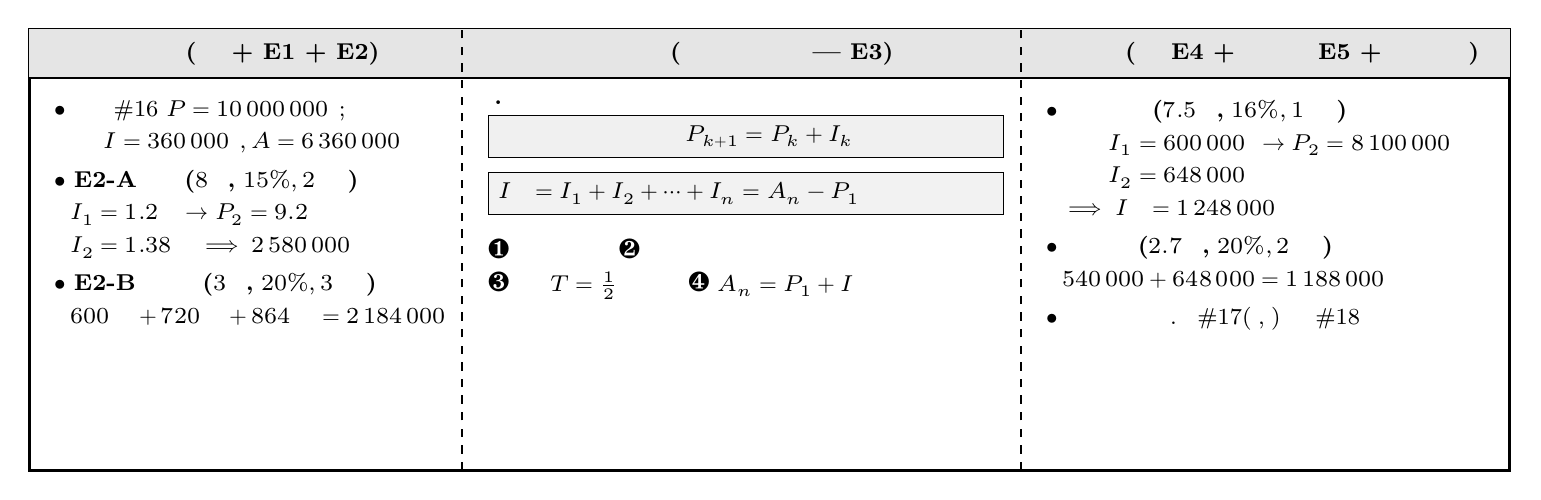
\begin{tikzpicture}[x=1cm, y=1cm, every node/.style={font=\fontsize{8.3pt}{11.8pt}\selectfont, text=black}]
  \draw[black, line width=1.1pt] (0,0) rectangle (18.8,5.60);
  \fill[gray!20] (0,4.98) rectangle (18.8,5.60);
  \draw[black, line width=0.7pt] (0,4.98) -- (18.8,4.98);
  \draw[black, dashed, line width=0.7pt] (5.5,0) -- (5.5,5.60);
  \draw[black, dashed, line width=0.7pt] (12.6,0) -- (12.6,5.60);

  \node at (2.75,5.29) {\textbf{ផ្នែកឆ្វេង (កំណែ + \en{E1} + \en{E2})}};
  \node at (9.05,5.29) {\textbf{ផ្នែកកណ្ដាល (ខ្លឹមសារគោលរក្សាទុក — \en{E3})}};
  \node at (15.70,5.29) {\textbf{ផ្នែកស្ដាំ (គំរូ \en{E4} + ប្រតិបត្តិ \en{E5} + កិច្ចការផ្ទះ)}};

  % Left
  \node[anchor=north west, text width=5.1cm] at (0.20,4.82) {%
    $\bullet$ \textbf{កំណែ៖} \#16 $P = 10\,000\,000\riel$;\\
    \hspace*{0.2cm}៩ខែ៖ $I = 360\,000\riel, A = 6\,360\,000\riel$\\[2pt]
    $\bullet$ \textbf{\en{E2-A} មីងសៅ ($8$លាន, $15\%, 2$ឆ្នាំ)៖}\\
    \hspace*{0.2cm}$I_1=1.2$លាន $\to P_2=9.2$លាន\\
    \hspace*{0.2cm}$I_2=1.38$លាន $\implies 2\,580\,000\riel$\\[2pt]
    $\bullet$ \textbf{\en{E2-B} ទ្រាចាន់ ($3$លាន, $20\%, 3$ឆ្នាំ)៖}\\
    \hspace*{0.2cm}$600\text{ពាន់}+720\text{ពាន់}+864\text{ពាន់}=2\,184\,000\riel$
  };

  % Center
  \node[anchor=north west, text width=6.7cm] at (5.70,4.82) {%
    {\muol\fontsize{8.5pt}{12pt}\selectfont ២\enbf{.}៦ ការប្រាក់សមាស}\\[3pt]
    \tikz\node[draw=black, fill=gray!12, inner sep=3.5pt, text width=6.3cm]{%
      បន្តប្រាក់ដើមថ្មីរាល់ដំណាក់៖ $P_{k+1} = P_k + I_k$
    };\\[4pt]
    \tikz\node[draw=black, fill=gray!10, inner sep=3.5pt, text width=6.3cm]{%
      $I_{\text{សមាស}} = I_1 + I_2 + \dots + I_n = A_n - P_1$
    };\\[4pt]
    \cnum{1} បន្តដើមថ្មី \quad \cnum{2} បូកគ្រប់ដំណាក់\\
    \cnum{3} ឆមាស $T=\frac{1}{2}$ ឆ្នាំ \quad \cnum{4} $A_n = P_1 + I_{\text{សមាស}}$
  };

  % Right
  \node[anchor=north west, text width=5.8cm] at (12.80,4.82) {%
    $\bullet$ \textbf{គំរូទី២ ឆមាស ($7.5$លាន, $16\%, 1$ឆ្នាំ)៖}\\
    \hspace*{0.2cm}ឆមាស១៖ $I_1 = 600\,000\riel \to P_2 = 8\,100\,000\riel$\\
    \hspace*{0.2cm}ឆមាស២៖ $I_2 = 648\,000\riel$\\
    \hspace*{0.2cm}$\implies I_{\text{សមាស}} = 1\,248\,000\riel$\\[2pt]
    $\bullet$ \textbf{ប្រតិបត្តិ ($2.7$លាន, $20\%, 2$ឆ្នាំ)៖}\\
    \hspace*{0.2cm}$540\,000 + 648\,000 = 1\,188\,000\riel$\\[2pt]
    $\bullet$ \textbf{កិច្ចការផ្ទះ៖} ទំ.៤២ \#17(ក,ខ) និង \#18
  };
\end{tikzpicture}
\end{center}

\vspace{4pt}
\secstrip{២. ចម្លើយផ្ទៀងផ្ទាត់រហ័សសម្រាប់សន្លឹកកិច្ចការសិស្ស \enbf{(}ទំព័រ ១ និង ទំព័រ ២\enbf{)}}{\en{Answer Key}}

\begin{tcolorbox}[
  enhanced, sharp corners, colback=white, colframe=black,
  boxrule=0.8pt, boxsep=2pt, top=4pt, bottom=4pt, left=6pt, right=6pt
]
  \fontsize{9.0pt}{13.6pt}\selectfont
  $\bullet$ \textbf{ផ្នែក \en{E1}៖} គណនី \en{B} បាន $210\,000\riel$; ដើមឆ្នាំទី២ ឡើងដល់ $1\,100\,000\riel$ ។\\[2pt]
  $\bullet$ \textbf{ផ្នែក \en{E2}៖} \textbf{សកម្មភាព ១ (មីងសៅ)៖} $P_2 = 9\,200\,000\riel, I_2 = 1\,380\,000\riel, A_2 = 10\,580\,000\riel \implies I_{\text{សមាស}} = 2\,580\,000\riel$ ។ \textbf{សកម្មភាព ២ (ទ្រាចាន់)៖} $I_2 = 720\,000\riel, A_2 = 4\,320\,000\riel$; $P_3 = 4\,320\,000\riel, I_3 = 864\,000\riel, A_3 = 5\,184\,000\riel \implies I_{\text{សមាស}} = 2\,184\,000\riel$ ។\\[2pt]
  $\bullet$ \textbf{ផ្នែក \en{E4}៖} $1$ ឆ្នាំ $= 2$ ឆមាស; $I_1 = 600\,000\riel \implies P_2 = 8\,100\,000\riel \implies I_2 = 648\,000\riel \implies I_{\text{សមាស}} = 1\,248\,000\riel$ ($8\%$ នៃ $600\,000\riel$) ។\\[2pt]
  $\bullet$ \textbf{ផ្នែក \en{E5}៖} \textbf{១) ប្រតិបត្តិ៖} $I_1 = 540\,000\riel, P_2 = 3\,240\,000\riel, I_2 = 648\,000\riel \implies 1\,188\,000\riel$ ។ \textbf{២) បិទ \en{E1}៖} $I_2 = 110\,000\riel \implies 210\,000\riel$ ។ \textbf{៣) វិនិច្ឆ័យ \en{A--D}៖} \textbf{ជម្រើស \en{C}} ($420\,000\riel$) ។ \textbf{៤) សំបុត្រចេញ៖} $200\,000\riel$, $1\,200\,000\riel$, $240\,000\riel \implies 440\,000\riel$ ។
\end{tcolorbox}

\vspace{4pt}
\secstrip{៣. ចម្លើយលម្អិតនៃកិច្ចការផ្ទះ \enbf{(}សម្រាប់ផ្ទៀងនៅដើមម៉ោងបន្ទាប់ ២\enbf{.}៧\enbf{)}}{សៀវភៅគោល ទំ.៤២}

\begin{tcolorbox}[
  enhanced, sharp corners, colback=white, colframe=black,
  boxrule=0.8pt, boxsep=2pt, top=4pt, bottom=4pt, left=6pt, right=6pt
]
  \fontsize{8.9pt}{13.4pt}\selectfont
  $\bullet$ \textbf{\#17 ក (ទំ.៤២ — $1\,800\,000\riel, 2$ ឆ្នាំ, $10\%$)៖} ឆ្នាំទី១ $I_1 = 180\,000\riel \implies P_2 = 1\,980\,000\riel$; ឆ្នាំទី២ $I_2 = 198\,000\riel \implies I_{\text{សមាស}} = 180\,000 + 198\,000 = \mathbf{378\,000\riel}$ ។\\[2pt]
  $\bullet$ \textbf{\#17 ខ (ទំ.៤២ — $2\,800\,000\riel, 3$ ឆ្នាំ, $11\%$)៖} ឆ្នាំទី១ $I_1 = 308\,000\riel \implies P_2 = 3\,108\,000\riel$; ឆ្នាំទី២ $I_2 = 341\,880\riel \implies P_3 = 3\,449\,880\riel$; ឆ្នាំទី៣ $I_3 = 379\,486.8\riel \implies I_{\text{សមាស}} = 308\,000 + 341\,880 + 379\,486.8 = \mathbf{1\,029\,366.8\riel}$ ។\\[2pt]
  $\bullet$ \textbf{\#18 (ទំ.៤២ — ពូសឿនឱ្យខ្ចី $20\,000\,000\riel, 15\%, 3$ ឆ្នាំ)៖} ឆ្នាំទី១ $I_1 = 3\,000\,000\riel \to P_2 = 23\,000\,000\riel$; ឆ្នាំទី២ $I_2 = 3\,450\,000\riel \to P_3 = 26\,450\,000\riel$; ឆ្នាំទី៣ $I_3 = 3\,967\,500\riel \implies$ \textbf{ប្រាក់សរុបដំណាច់ឆ្នាំទី៣} $A_3 = 26\,450\,000 + 3\,967\,500 = \mathbf{30\,417\,500\riel}$ ។
\end{tcolorbox}

\end{document}
